\documentclass{article}
\usepackage{graphics} 
\usepackage{hyperref}

\author{Kevin Zollicoffer}
\title{Predictive Modeling\\Lesson 3\\\emph{Logistical Regression and Neural Networks}}
\date{09/29/2013}

\usepackage{Sweave}
\begin{document}
\maketitle
%\tableofcontents
\Sconcordance{concordance:LogisticalRegression.tex:LogisticalRegression.Rnw:%
1 8 1 1 0 15 1 1 2 1 0 1 1 40 0 1 2 2 1 1 2 1 0 5 1 3 0 1 2 2 1 1 2 1 0 %
3 1 3 0 1 2 3 1 1 2 1 0 1 2 39 0 1 2 73 0 1 2 49 0 1 2 208 0 1 3 2 1 1 %
2 1 0 1 1 7 0 1 2 2 1 1 2 1 0 2 1 36 0 1 2 1 1 1 2 1 0 3 1 3 0 1 2 3 1 %
1 2 1 0 1 1 3 0 1 2 2 1 1 9 7 0 1 6 4 0 2 1 401 0 1 2 17 1}


\section*{Introduction}
I chose to use R for the assignments. This is my first class in the PASS program and one of my goals upon completion of PASS is to be proficient in R. 
\\
\\
\noindent
The RStudio project files and accompanying artifacts, including the tex file that created this PDF, are publicly available on GitHub
\\
\url{https://github.com/zollie/PASS-PredictiveModeling-LogisticalRegression}

\section*{Data Setup}
I took the Excel spreadsheet and saved it as a CSV for easy import into R
\begin{Schunk}
\begin{Sinput}
> gc <- read.csv("~/R/PASS/PredictiveModeling/LogisticRegression/GermanCredit.csv")
> head(gc)
\end{Sinput}
\begin{Soutput}
  OBS. CHK_ACCT DURATION HISTORY NEW_CAR USED_CAR FURNITURE RADIO.TV EDUCATION
1    1        0        6       4       0        0         0        1         0
2    2        1       48       2       0        0         0        1         0
3    3        3       12       4       0        0         0        0         1
4    4        0       42       2       0        0         1        0         0
5    5        0       24       3       1        0         0        0         0
6    6        3       36       2       0        0         0        0         1
  RETRAINING AMOUNT SAV_ACCT EMPLOYMENT INSTALL_RATE MALE_DIV MALE_SINGLE
1          0   1169        4          4            4        0           1
2          0   5951        0          2            2        0           0
3          0   2096        0          3            2        0           1
4          0   7882        0          3            2        0           1
5          0   4870        0          2            3        0           1
6          0   9055        4          2            2        0           1
  MALE_MAR_or_WID CO.APPLICANT GUARANTOR PRESENT_RESIDENT REAL_ESTATE
1               0            0         0                4           1
2               0            0         0                2           1
3               0            0         0                3           1
4               0            0         1                4           0
5               0            0         0                4           0
6               0            0         0                4           0
  PROP_UNKN_NONE AGE OTHER_INSTALL RENT OWN_RES NUM_CREDITS JOB NUM_DEPENDENTS
1              0  67             0    0       1           2   2              1
2              0  22             0    0       1           1   2              1
3              0  49             0    0       1           1   1              2
4              0  45             0    0       0           1   2              2
5              1  53             0    0       0           2   2              2
6              1  35             0    0       0           1   1              2
  TELEPHONE FOREIGN RESPONSE
1         1       0        1
2         0       0        0
3         0       0        1
4         0       0        1
5         0       0        0
6         1       0        1
\end{Soutput}
\end{Schunk}

\noindent
The categorical predictors are turned into factors for R
\begin{Schunk}
\begin{Sinput}
> gc$RESPONSE <- factor(gc$RESPONSE)
> gc$JOB <- factor(gc$JOB)
> gc$EMPLOYMENT <- factor(gc$EMPLOYMENT)
> gc$SAV_ACCT <- factor(gc$SAV_ACCT)
> gc$HISTORY <- factor(gc$HISTORY)
> gc$CHK_ACCT <- factor(gc$CHK_ACCT)
\end{Sinput}
\end{Schunk}

\section*{Partitioning}
Next, the data is paritioned into 60\% Train and 40\% Test sets. I set the RNG seed for reproducibility
\begin{Schunk}
\begin{Sinput}
> n <- nrow(gc)
> a <- sort(sample(1:n, floor(n*.6)))
> gc.train <- gc[a,]
> gc.test <- gc[-a,]
\end{Sinput}
\end{Schunk}

\section*{Logistical Regression}
A Logistical Regression model is fit to the train data. 

\begin{Schunk}
\begin{Sinput}
> logit <- glm(RESPONSE ~ CHK_ACCT+DURATION+HISTORY+NEW_CAR+USED_CAR+FURNITURE+RADIO.TV+EDUCATION+RETRAINING+AMOUNT+SAV_ACCT+EMPLOYMENT+INSTALL_RATE+MALE_DIV+MALE_SINGLE+MALE_MAR_or_WID+CO.APPLICANT+GUARANTOR+PRESENT_RESIDENT+REAL_ESTATE+PROP_UNKN_NONE+AGE+OTHER_INSTALL+RENT+OWN_RES+NUM_CREDITS+JOB+NUM_DEPENDENTS+TELEPHONE+FOREIGN, data=gc.train, family=binomial("logit"))
> logit
\end{Sinput}
\begin{Soutput}
Call:  glm(formula = RESPONSE ~ CHK_ACCT + DURATION + HISTORY + NEW_CAR + 
    USED_CAR + FURNITURE + RADIO.TV + EDUCATION + RETRAINING + 
    AMOUNT + SAV_ACCT + EMPLOYMENT + INSTALL_RATE + MALE_DIV + 
    MALE_SINGLE + MALE_MAR_or_WID + CO.APPLICANT + GUARANTOR + 
    PRESENT_RESIDENT + REAL_ESTATE + PROP_UNKN_NONE + AGE + OTHER_INSTALL + 
    RENT + OWN_RES + NUM_CREDITS + JOB + NUM_DEPENDENTS + TELEPHONE + 
    FOREIGN, family = binomial("logit"), data = gc.train)

Coefficients:
     (Intercept)         CHK_ACCT1         CHK_ACCT2         CHK_ACCT3  
      -0.0785683         0.3782587         1.3235863         1.8611904  
        DURATION          HISTORY1          HISTORY2          HISTORY3  
      -0.0367290         0.2115982         1.0612918         1.8523658  
        HISTORY4           NEW_CAR          USED_CAR         FURNITURE  
       2.3108484        -0.7254331         1.0471379         0.3166340  
        RADIO.TV         EDUCATION        RETRAINING            AMOUNT  
       0.3402443        -1.1564688         0.0332020        -0.0001519  
       SAV_ACCT1         SAV_ACCT2         SAV_ACCT3         SAV_ACCT4  
       0.5192510        -0.1274285         1.8195726         1.0523181  
     EMPLOYMENT1       EMPLOYMENT2       EMPLOYMENT3       EMPLOYMENT4  
       0.6200766         0.5109157         1.3376031         0.7209663  
    INSTALL_RATE          MALE_DIV       MALE_SINGLE   MALE_MAR_or_WID  
      -0.3366400        -0.7343612         0.2732063         0.1828317  
    CO.APPLICANT         GUARANTOR  PRESENT_RESIDENT       REAL_ESTATE  
      -0.6144330         0.8224780         0.0885999        -0.1658967  
  PROP_UNKN_NONE               AGE     OTHER_INSTALL              RENT  
      -0.2548482         0.0116311        -0.5959307        -0.1989817  
         OWN_RES       NUM_CREDITS              JOB1              JOB2  
       0.2276633        -0.2794957        -0.2758346        -0.3001333  
            JOB3    NUM_DEPENDENTS         TELEPHONE           FOREIGN  
       0.1589518        -0.0448547         0.0783900         2.2237732  

Degrees of Freedom: 599 Total (i.e. Null);  556 Residual
Null Deviance:	    746.1 
Residual Deviance: 505.8 	AIC: 593.8
\end{Soutput}
\begin{Sinput}
> summary(logit)
\end{Sinput}
\begin{Soutput}
Call:
glm(formula = RESPONSE ~ CHK_ACCT + DURATION + HISTORY + NEW_CAR + 
    USED_CAR + FURNITURE + RADIO.TV + EDUCATION + RETRAINING + 
    AMOUNT + SAV_ACCT + EMPLOYMENT + INSTALL_RATE + MALE_DIV + 
    MALE_SINGLE + MALE_MAR_or_WID + CO.APPLICANT + GUARANTOR + 
    PRESENT_RESIDENT + REAL_ESTATE + PROP_UNKN_NONE + AGE + OTHER_INSTALL + 
    RENT + OWN_RES + NUM_CREDITS + JOB + NUM_DEPENDENTS + TELEPHONE + 
    FOREIGN, family = binomial("logit"), data = gc.train)

Deviance Residuals: 
    Min       1Q   Median       3Q      Max  
-2.9087  -0.6148   0.3155   0.6546   2.8146  

Coefficients:
                   Estimate Std. Error z value Pr(>|z|)    
(Intercept)      -0.0785683  1.5781963  -0.050  0.96029    
CHK_ACCT1         0.3782587  0.2961859   1.277  0.20157    
CHK_ACCT2         1.3235862  0.5028576   2.632  0.00849 ** 
CHK_ACCT3         1.8611903  0.3100238   6.003 1.93e-09 ***
DURATION         -0.0367290  0.0124796  -2.943  0.00325 ** 
HISTORY1          0.2115982  0.8101723   0.261  0.79396    
HISTORY2          1.0612918  0.6572103   1.615  0.10634    
HISTORY3          1.8523658  0.7191174   2.576  0.01000 ** 
HISTORY4          2.3108484  0.6716128   3.441  0.00058 ***
NEW_CAR          -0.7254331  0.5221924  -1.389  0.16477    
USED_CAR          1.0471379  0.6759156   1.549  0.12133    
FURNITURE         0.3166340  0.5519902   0.574  0.56622    
RADIO.TV          0.3402443  0.5207861   0.653  0.51354    
EDUCATION        -1.1564688  0.6739694  -1.716  0.08618 .  
RETRAINING        0.0332020  0.5901414   0.056  0.95513    
AMOUNT           -0.0001519  0.0000618  -2.458  0.01399 *  
SAV_ACCT1         0.5192510  0.4045415   1.284  0.19930    
SAV_ACCT2        -0.1274285  0.4957171  -0.257  0.79713    
SAV_ACCT3         1.8195726  0.7633959   2.384  0.01715 *  
SAV_ACCT4         1.0523181  0.3564120   2.953  0.00315 ** 
EMPLOYMENT1       0.6200766  0.5617987   1.104  0.26971    
EMPLOYMENT2       0.5109157  0.5377445   0.950  0.34206    
EMPLOYMENT3       1.3376031  0.6023203   2.221  0.02637 *  
EMPLOYMENT4       0.7209663  0.5458410   1.321  0.18656    
INSTALL_RATE     -0.3366400  0.1267726  -2.655  0.00792 ** 
MALE_DIV         -0.7343612  0.5379059  -1.365  0.17218    
MALE_SINGLE       0.2732063  0.2838544   0.962  0.33580    
MALE_MAR_or_WID   0.1828317  0.4285412   0.427  0.66964    
CO.APPLICANT     -0.6144330  0.5734994  -1.071  0.28400    
GUARANTOR         0.8224780  0.5575590   1.475  0.14017    
PRESENT_RESIDENT  0.0885999  0.1206828   0.734  0.46285    
REAL_ESTATE      -0.1658967  0.2918338  -0.568  0.56972    
PROP_UNKN_NONE   -0.2548482  0.5198569  -0.490  0.62397    
AGE               0.0116311  0.0125096   0.930  0.35249    
OTHER_INSTALL    -0.5959307  0.2868482  -2.078  0.03775 *  
RENT             -0.1989817  0.6446811  -0.309  0.75759    
OWN_RES           0.2276633  0.5896176   0.386  0.69941    
NUM_CREDITS      -0.2794957  0.2585156  -1.081  0.27963    
JOB1             -0.2758346  0.9027783  -0.306  0.75996    
JOB2             -0.3001333  0.8651196  -0.347  0.72865    
JOB3              0.1589518  0.8771417   0.181  0.85620    
NUM_DEPENDENTS   -0.0448547  0.3311909  -0.135  0.89227    
TELEPHONE         0.0783901  0.2718810   0.288  0.77310    
FOREIGN           2.2237732  0.9811973   2.266  0.02343 *  
---
Signif. codes:  0 ‘***’ 0.001 ‘**’ 0.01 ‘*’ 0.05 ‘.’ 0.1 ‘ ’ 1

(Dispersion parameter for binomial family taken to be 1)

    Null deviance: 746.09  on 599  degrees of freedom
Residual deviance: 505.78  on 556  degrees of freedom
AIC: 593.78

Number of Fisher Scoring iterations: 5
\end{Soutput}
\begin{Sinput}
> confint(logit)
\end{Sinput}
\begin{Soutput}
                         2.5 %        97.5 %
(Intercept)      -3.2063351906  3.002071e+00
CHK_ACCT1        -0.2015859939  9.617137e-01
CHK_ACCT2         0.3706373386  2.357903e+00
CHK_ACCT3         1.2649147013  2.483309e+00
DURATION         -0.0615291292 -1.245575e-02
HISTORY1         -1.3543807890  1.849954e+00
HISTORY2         -0.1732084618  2.433398e+00
HISTORY3          0.4977459146  3.343435e+00
HISTORY4          1.0548571647  3.717226e+00
NEW_CAR          -1.7738796827  2.845090e-01
USED_CAR         -0.2635782167  2.400403e+00
FURNITURE        -0.7823098999  1.392642e+00
RADIO.TV         -0.7018959248  1.352020e+00
EDUCATION        -2.5004504936  1.522616e-01
RETRAINING       -1.1339491571  1.190497e+00
AMOUNT           -0.0002757537 -3.240653e-05
SAV_ACCT1        -0.2581830784  1.333756e+00
SAV_ACCT2        -1.0662554758  8.964553e-01
SAV_ACCT3         0.4613739482  3.521840e+00
SAV_ACCT4         0.3728669872  1.774989e+00
EMPLOYMENT1      -0.4800061097  1.731419e+00
EMPLOYMENT2      -0.5423158477  1.575124e+00
EMPLOYMENT3       0.1679229661  2.538261e+00
EMPLOYMENT4      -0.3539151781  1.793599e+00
INSTALL_RATE     -0.5894593436 -9.138965e-02
MALE_DIV         -1.8084035624  3.129979e-01
MALE_SINGLE      -0.2845760285  8.305893e-01
MALE_MAR_or_WID  -0.6459920388  1.041097e+00
CO.APPLICANT     -1.7562837391  5.090849e-01
GUARANTOR        -0.2182255182  1.996404e+00
PRESENT_RESIDENT -0.1474113942  3.266883e-01
REAL_ESTATE      -0.7378036695  4.087772e-01
PROP_UNKN_NONE   -1.2648083616  7.809314e-01
AGE              -0.0126216177  3.656521e-02
OTHER_INSTALL    -1.1598786021 -3.259447e-02
RENT             -1.4644289302  1.070742e+00
OWN_RES          -0.9265735081  1.394243e+00
NUM_CREDITS      -0.7955882483  2.235612e-01
JOB1             -2.0578340242  1.511506e+00
JOB2             -2.0104097095  1.413896e+00
JOB3             -1.5706981657  1.902724e+00
NUM_DEPENDENTS   -0.6903890299  6.115326e-01
TELEPHONE        -0.4536461112  6.146903e-01
FOREIGN           0.5601694533  4.550100e+00
\end{Soutput}
\begin{Sinput}
> residuals(logit)
\end{Sinput}
\begin{Soutput}
          1           2           3           4           5           9 
 0.27658938 -0.70745956  0.26031200  0.96285619 -0.78091812  0.14471802 
         10          17          19          20          23          24 
-0.82960779  0.17438277 -0.91198870  0.54979701  0.29479334  0.20880762 
         25          27          29          30          31          33 
 0.04862382  0.54535137  0.58357349 -0.72045864  0.59020983  1.33280097 
         35          38          39          40          41          42 
 0.71014300 -1.15142024  0.46878252  0.89028073  0.71277786  1.26500871 
         45          46          49          50          51          53 
-0.88196827  0.38400917  0.40302983  0.65273665  0.67054505  0.41731826 
         55          57          60          61          62          63 
-0.71142399 -1.84894169 -0.58102823  1.09571430  0.20410459 -0.82032605 
         64          65          67          68          70          71 
-0.26134110  0.65463696  0.53238217  0.79480171  0.51257570  0.77759519 
         73          74          75          76          77          79 
 0.65465975  1.17197065 -1.01655513  0.36474180 -0.78791273  0.86514710 
         80          82          83          86          87          90 
 1.14738766  0.53610483  0.54485543  0.22452247  0.76826154 -0.90758986 
         91          95          98          99         100         103 
 0.19149555  0.51339005  0.91856030  0.74770385  0.37618695  0.31052324 
        104         105         106         107         112         115 
 0.39774409  0.17489301 -1.15545192 -1.06157760  1.31169279  1.04227288 
        116         117         118         119         122         123 
 0.31506449 -1.39110675  0.21273095 -1.47600155  0.29187104  0.57482794 
        125         126         128         130         134         136 
-1.45869141  1.16412454 -1.34690556 -0.82376254  0.86801372  0.18250831 
        137         138         142         143         145         146 
 0.17883779 -1.59778633  1.50897246  1.11848700  0.33238714  1.55174344 
        147         150         152         155         157         159 
 0.63600164  0.10423581  0.08280896  0.63001846  0.10071723  1.09729601 
        161         162         163         166         167         168 
 0.20385032  0.61163007  0.43201213  0.30586163 -0.89212366  0.53152738 
        169         170         171         172         174         177 
 0.44975955 -1.20280356 -0.42687108  0.58599551  0.22378190  1.28490783 
        178         179         180         182         184         185 
 0.47977999  0.37184174  0.94885291 -0.76307521  0.13701741 -1.41864831 
        186         187         188         189         190         192 
 0.31551697 -1.49846060  0.80153818 -1.79906631  1.53891593 -0.66980377 
        193         195         198         202         205         206 
-0.96526654 -1.23852387 -0.89641647  1.60813038  0.50014714  1.01327815 
        207         208         211         213         216         218 
 0.29192076  0.41890859  0.12739240 -0.39742634  0.15862334  0.86105846 
        219         220         222         225         226         230 
 1.82087954  0.46676765  1.75519087  0.37585140  1.47818274  1.90841083 
        231         232         233         234         236         237 
-1.26573361  0.58110397  0.25846246  0.78888305 -0.80481474 -1.02085472 
        238         241         242         243         244         245 
-0.65625559 -0.85623352  0.22640693 -0.48529569  0.36843929  1.11171267 
        247         249         250         252         257         258 
 0.26014723  0.64137567 -1.37520741  0.42594979  0.42712958 -0.43354974 
        260         262         264         265         266         267 
 0.31987808  1.10624197  0.74692643  0.12268555 -1.58933228  0.40146481 
        268         269         272         274         276         277 
 0.74602482 -1.74291754  0.19086916 -1.00329205  0.33809349  0.30444485 
        280         281         284         285         287         290 
 0.42145952  0.10362142  0.11482208  1.27993411  1.20707179 -1.30165165 
        291         293         295         296         298         299 
 0.14772632  0.58714471  0.87903772 -0.74061907  0.17312917  0.44515219 
        300         302         304         305         307         308 
 0.18033341 -0.54371133  0.83672917 -0.88479280  0.30966495 -1.55209656 
        313         314         318         319         320         322 
 0.67027653 -1.40738769  0.50847968  0.57917072  0.66784523 -0.76715954 
        323         324         326         328         330         331 
 0.55669546  0.60713462  0.17382553  0.29484221  0.72416258  0.60685833 
        332         333         336         337         338         342 
-1.78253077 -0.42036804 -1.91909686  0.52226782 -1.21487496  0.84717397 
        345         346         350         351         354         355 
 0.48190735  0.29248498 -1.99908877  0.43298493 -0.45742320  0.85490034 
        356         357         358         359         362         363 
-0.61255931  0.10624364 -1.95612423  0.52482009  0.20815767  0.85088734 
        364         366         369         370         372         374 
 0.37362324  0.23283687 -0.90739846  0.77289123  0.31551224  0.93627090 
        375         376         377         381         382         384 
-0.20297565 -0.68940640  0.43915324  0.49562406 -0.86905023  1.04764469 
        389         390         391         392         394         397 
 0.66435632  0.40315692  0.53587566  0.34345458  0.25952823  1.16426422 
        398         399         400         401         402         403 
 0.90977940 -0.79623044  0.18341525  0.41355789  0.68279115 -1.61644921 
        404         405         406         407         408         410 
 0.62035251  0.65270465 -1.62172971  0.09242299  0.45394345 -1.95593668 
        411         413         414         416         418         419 
 1.10861081 -2.14520566  0.32369106  0.28357706  1.47800030  0.55254468 
        420         425         427         428         430         431 
-1.26215725 -1.97967151  0.40210989  0.12715224 -1.40835571  0.17946231 
        432         433         437         440         444         445 
-0.53388322  0.84607433  0.32731930 -1.33295866 -1.44185872 -1.61310120 
        446         448         449         452         454         456 
 0.37911206  0.50200140  0.22121141  0.44782547  0.28914759  0.46107648 
        457         459         460         462         463         464 
 1.21895191  1.25313944  0.51829573  1.26919320  1.03580558  0.59937721 
        466         468         469         470         471         472 
 0.73395686  0.64322773  0.56459984  0.21137877 -1.32936674 -0.80398595 
        473         474         475         477         478         479 
-0.96750682  0.27134597 -1.89413388  0.60223636  0.88984645  0.46156503 
        480         483         485         487         490         491 
 0.59424048  0.84926766  0.40830999  0.30753765  0.49401828  0.23582057 
        492         494         495         497         498         499 
-0.59197657  0.39256946  0.48449219 -0.58462577  0.23140910  0.71511220 
        500         505         506         509         511         512 
 0.44153756 -0.57293692 -2.53068672  0.62290415 -1.12790093  0.46379636 
        513         514         516         520         522         524 
 0.45200597  1.17162970  0.25265169  0.15458017 -1.13886538  0.23777402 
        527         528         530         531         532         533 
 0.48831145  0.13387234  1.11601821  1.67583269 -1.05191108  0.28237128 
        534         535         536         537         540         542 
 0.30473612  0.45371867 -1.23624146  0.85691673  0.65631890  0.68235657 
        543         546         548         549         552         554 
-1.28576342 -0.62148321  0.48270423 -0.66425374  0.52644720  0.72145806 
        556         560         561         562         564         565 
-1.45396463 -2.02523307  0.83277765 -1.04575434 -0.76313979  0.80837536 
        568         570         572         574         575         576 
 0.09135836 -0.56711333  0.37194029  1.28757402  0.83643062  0.35062432 
        578         579         583         586         587         589 
 0.44148240 -0.68380329  0.70239603 -0.97550463  1.11680340 -1.10877016 
        590         593         594         595         598         599 
-2.07897031  0.36070894 -0.69690045 -1.18633590 -0.79455415 -2.26639741 
        600         601         602         604         608         609 
 0.43349472  0.44861157 -1.35693800 -1.68264442 -0.82571293  0.58787776 
        610         614         615         616         617         621 
 0.28263687  0.46755342 -2.38679918  1.99377185  1.12189242  0.46747352 
        623         625         628         632         633         635 
-0.95926779 -1.03529827 -1.46078579 -0.71772556  0.63776132 -0.97740611 
        636         637         639         641         642         643 
 1.14968053  0.50984645  0.50153632 -0.46826358  1.01159550 -1.84952698 
        644         645         646         648         649         650 
 0.16993871  0.47576021 -1.78993395 -1.73775199 -1.18058400 -0.69267485 
        652         653         655         656         657         658 
-1.44835076 -0.53008626  0.16897341  1.70748179 -0.98365429  0.80277651 
        660         661         662         664         665         666 
 0.60285443  0.68653237 -1.23190775  0.87002640  0.41255199  1.14914539 
        667         669         671         673         675         676 
 1.14964957 -0.98554370  0.32472288  1.33146101 -1.79988115  0.31085982 
        677         678         679         680         682         683 
 0.34130062 -0.72764296  1.50122154  0.56848880  0.33195574  0.56386267 
        685         688         690         692         694         695 
 0.73613583  1.36373325  0.57561702  1.02873524  0.48202914  0.41584836 
        696         699         700         703         704         706 
 0.23462742  0.35775167  0.97728201  0.67218530  1.07246472  0.82671055 
        707         709         710         712         713         715 
-0.81069607  0.91868281  0.73072758 -0.46518635  0.16354207 -0.30313679 
        716         718         722         723         725         726 
 0.11555637  0.51831747 -0.84501520 -0.69808440 -1.07659091  0.18985286 
        727         729         730         736         737         738 
 0.22678159 -0.32023581  0.25049186  1.70506865 -1.14500858  1.33055769 
        739         741         742         743         745         746 
 0.21607930  1.49662760  1.50779983  0.30315521  0.84572786  0.94880181 
        747         749         750         752         755         757 
 1.71664471  0.19110212  0.19224839 -1.09521451 -2.90872649  0.10663956 
        758         759         761         763         766         767 
-2.73148775  0.50096642  0.17170266  1.11194008  0.75195413 -0.89073659 
        768         770         772         773         774         775 
 0.17735006  0.15543588 -0.52897397  0.09291075  0.30148054  0.78295435 
        776         777         778         781         782         787 
-0.80522715  0.51338444  0.87631007 -2.12819265  0.17023610  0.44778048 
        788         790         792         794         795         796 
 0.21832556 -0.40568134  0.18916837  1.03397628  0.80099346  0.35488968 
        797         798         799         800         801         802 
-2.18657401  0.27492340  0.32519154  0.79477089  0.71316952  0.57897504 
        803         804         806         807         810         811 
 0.63265210  0.13934863 -0.63868306  0.25151462 -0.53352786  0.87930771 
        813         814         815         816         817         818 
-1.52801395 -0.83171030 -0.53462389  1.71291985  0.44860657  0.15544183 
        819         820         822         823         824         825 
 2.81456332 -0.86667570  0.66320680 -0.97473804  0.84977604  0.39795181 
        826         827         828         830         833         836 
 1.14939605 -0.89800164 -1.14019601  1.24257689 -0.23414053 -0.43070659 
        837         838         839         843         845         846 
 0.33533451  0.35561301  0.48392557 -1.71988917  0.78807811  0.37008374 
        847         849         850         852         853         854 
-1.90472574  0.53691092 -1.30945283  0.08786790  0.34729786 -0.58974541 
        855         857         858         859         860         861 
 1.04714294  0.21068372  0.39894702 -0.72633562  0.13436345  0.16550501 
        862         863         865         866         867         868 
-2.15101981 -1.02156006 -1.83378359  0.56711148  1.62858240  0.22827346 
        870         873         877         878         879         881 
 1.20124980  0.61069334  1.79052178  0.76813641 -1.07061071  0.27285037 
        883         886         887         888         889         890 
 0.76374008 -0.83033534  0.41407405 -0.39495832  0.69429616  0.61447649 
        891         892         893         895         896         897 
 1.14932262  0.23868163  0.51672304  0.18220260  0.22189564  1.25323656 
        898         900         901         902         903         904 
 0.02244865 -1.11914811 -1.70057193  0.40273506  0.27120371  0.38707984 
        905         908         909         914         915         916 
 0.45018241  1.40206672  0.19734416  0.22812122 -0.51216097 -0.56106481 
        917         919         920         921         922         924 
 0.25808906 -1.00638500 -1.13620438  0.45646527  0.76719296  1.01093491 
        925         926         927         928         929         931 
-0.40704126 -0.48661939  0.86974843 -0.45293580  0.28139959  0.69309498 
        932         933         937         938         939         940 
-1.39808538  0.45386760 -1.91887727  0.80774257 -0.23763055  0.11086880 
        941         943         947         948         950         951 
 0.26922394  0.30008460 -0.58905277  0.52683815 -2.32422726  0.89090328 
        954         955         959         961         962         963 
-0.84927884  1.22483217 -0.70132021  0.25162909  1.19332642  0.57481093 
        964         966         971         972         973         974 
-1.70437458  0.95454931  0.71619855  0.79193131 -0.31599589 -0.23588197 
        975         978         979         982         983         984 
 0.43529989  0.54172931 -1.84219539 -0.90570290  0.78537806 -1.01555782 
        986         988         992         993         998        1000 
 1.01359888  0.33134949  0.64958275  0.55043387  0.36621902  0.67473182 
\end{Soutput}
\begin{Sinput}
> 
\end{Sinput}
\end{Schunk}

\subsection*{Using the model with the test data}
The test data is then run through the model
\begin{Schunk}
\begin{Sinput}
> p.test <- predict(logit, gc.test, type="response")
> summary(p.test)
\end{Sinput}
\begin{Soutput}
   Min. 1st Qu.  Median    Mean 3rd Qu.    Max. 
0.01537 0.48390 0.76120 0.68070 0.92110 0.99980 
\end{Soutput}
\end{Schunk}

\subsection*{Classification Table}
A baseline Classification Table with cutoff = 50\% is given
\begin{Schunk}
\begin{Sinput}
> library(gmodels)
> p.test.vals <- sapply(p.test, function(y) { ifelse(y<.5,0, 1) })
> CrossTable(gc.test$RESPONSE, p.test.vals, dnn = c("Actual", "Predicted"))
\end{Sinput}
\begin{Soutput}
   Cell Contents
|-------------------------|
|                       N |
| Chi-square contribution |
|           N / Row Total |
|           N / Col Total |
|         N / Table Total |
|-------------------------|

 
Total Observations in Table:  400 

 
             | Predicted 
      Actual |         0 |         1 | Row Total | 
-------------|-----------|-----------|-----------|
           0 |        56 |        56 |       112 | 
             |    25.578 |     8.870 |           | 
             |     0.500 |     0.500 |     0.280 | 
             |     0.544 |     0.189 |           | 
             |     0.140 |     0.140 |           | 
-------------|-----------|-----------|-----------|
           1 |        47 |       241 |       288 | 
             |     9.947 |     3.450 |           | 
             |     0.163 |     0.837 |     0.720 | 
             |     0.456 |     0.811 |           | 
             |     0.117 |     0.603 |           | 
-------------|-----------|-----------|-----------|
Column Total |       103 |       297 |       400 | 
             |     0.258 |     0.743 |           | 
-------------|-----------|-----------|-----------|
\end{Soutput}
\end{Schunk}

\subsection*{ROC Curve}
\begin{Schunk}
\begin{Sinput}
> library(ROCR)
> p.rocr <- prediction(p.test, gc.test$RESPONSE)
> p.rocr.roc <- performance(p.rocr, "tpr", "fpr")
> plot(p.rocr.roc, main="ROC Curve", colorize=T)
\end{Sinput}
\end{Schunk}
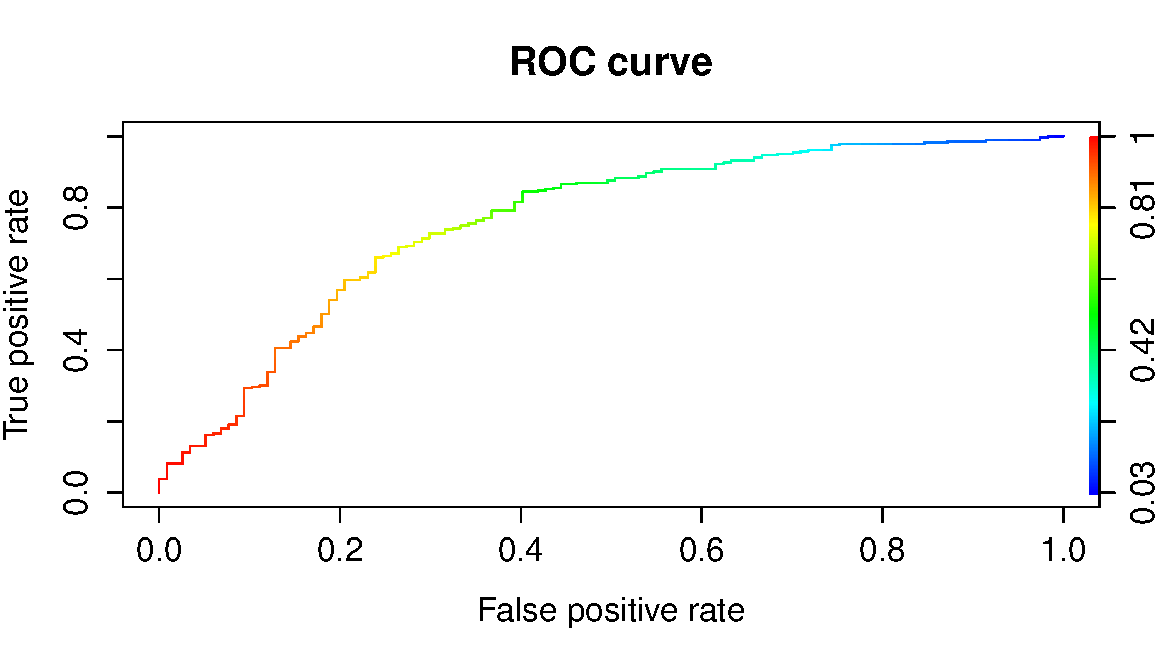
\includegraphics[width=0.98\textwidth]{ROCCurve.pdf}


\subsection*{Lift Curve}
\begin{Schunk}
\begin{Sinput}
> p.rocr.lift <- performance(p.rocr, "lift", "rpp")
> plot(p.rocr.lift, main="Lift Curve", colorize=T)
\end{Sinput}
\end{Schunk}
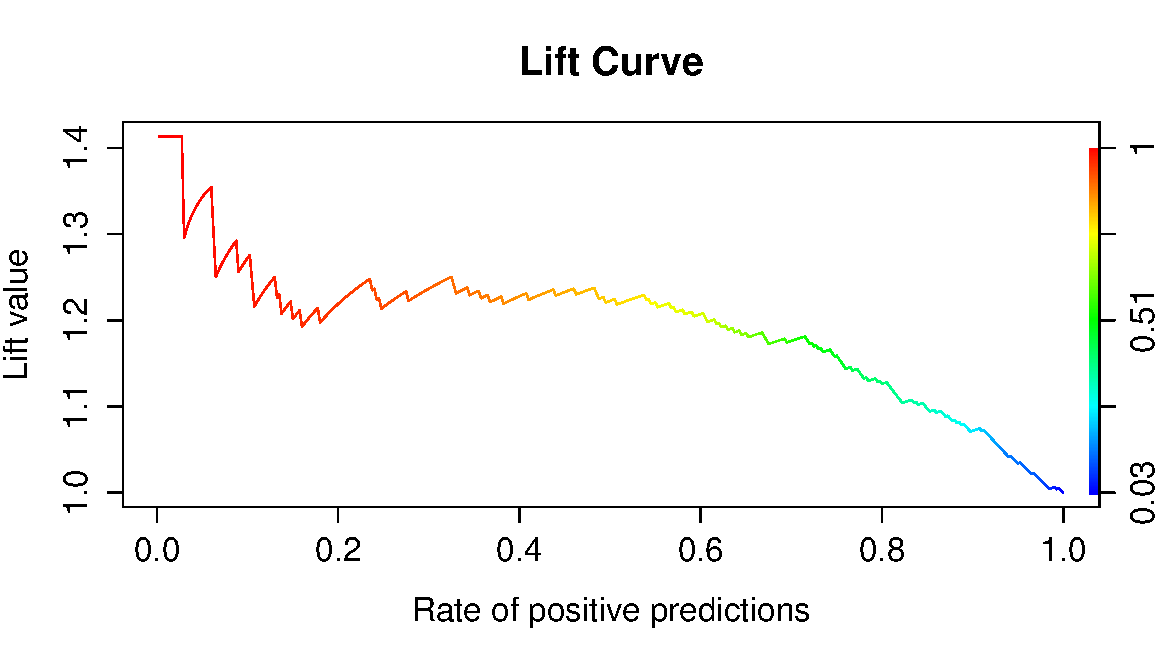
\includegraphics[width=0.98\textwidth]{LiftCurve.pdf}

\subsection{Classification Table with different cutoff values}
\begin{Schunk}
\begin{Sinput}
> calcNetProfit <- function(facts, preds, cutoff) {
+   vals <- sapply(preds, function(y) { ifelse(y<cutoff,0, 1) })  
+   ct <- CrossTable(facts, vals, dnn = c("Actual", "Predicted"))
+   print("Profit with cutoff")
+   print(cutoff)
+   profitFromCrossTable(ct)
+ }
> profitFromCrossTable <- function(ct) {
+   profit <- ct$t[1,1] * 100
+   loss <- ct$t[2,1] * -500
+   profit - loss
+ }
> s <- seq(0,1, by = .1)
> for(i in s) { print(calcNetProfit(gc.test$RESPONSE, p.test, i)) }
\end{Sinput}
\begin{Soutput}
   Cell Contents
|-------------------------|
|                       N |
|         N / Table Total |
|-------------------------|

 
Total Observations in Table:  400 

 
             | vals 
       facts |         1 | Row Total | 
-------------|-----------|-----------|
           0 |       112 |       112 | 
             |     0.280 |           | 
-------------|-----------|-----------|
           1 |       288 |       288 | 
             |     0.720 |           | 
-------------|-----------|-----------|
Column Total |       400 |       400 | 
-------------|-----------|-----------|

 
[1] "Profit with cutoff"
[1] 0
[1] 155200

 
   Cell Contents
|-------------------------|
|                       N |
| Chi-square contribution |
|           N / Row Total |
|           N / Col Total |
|         N / Table Total |
|-------------------------|

 
Total Observations in Table:  400 

 
             | Predicted 
      Actual |         0 |         1 | Row Total | 
-------------|-----------|-----------|-----------|
           0 |         8 |       104 |       112 | 
             |     5.222 |     0.175 |           | 
             |     0.071 |     0.929 |     0.280 | 
             |     0.615 |     0.269 |           | 
             |     0.020 |     0.260 |           | 
-------------|-----------|-----------|-----------|
           1 |         5 |       283 |       288 | 
             |     2.031 |     0.068 |           | 
             |     0.017 |     0.983 |     0.720 | 
             |     0.385 |     0.731 |           | 
             |     0.013 |     0.708 |           | 
-------------|-----------|-----------|-----------|
Column Total |        13 |       387 |       400 | 
             |     0.033 |     0.968 |           | 
-------------|-----------|-----------|-----------|

 
[1] "Profit with cutoff"
[1] 0.1
[1] 3300

 
   Cell Contents
|-------------------------|
|                       N |
| Chi-square contribution |
|           N / Row Total |
|           N / Col Total |
|         N / Table Total |
|-------------------------|

 
Total Observations in Table:  400 

 
             | Predicted 
      Actual |         0 |         1 | Row Total | 
-------------|-----------|-----------|-----------|
           0 |        21 |        91 |       112 | 
             |    14.967 |     1.346 |           | 
             |     0.188 |     0.812 |     0.280 | 
             |     0.636 |     0.248 |           | 
             |     0.052 |     0.228 |           | 
-------------|-----------|-----------|-----------|
           1 |        12 |       276 |       288 | 
             |     5.821 |     0.523 |           | 
             |     0.042 |     0.958 |     0.720 | 
             |     0.364 |     0.752 |           | 
             |     0.030 |     0.690 |           | 
-------------|-----------|-----------|-----------|
Column Total |        33 |       367 |       400 | 
             |     0.083 |     0.917 |           | 
-------------|-----------|-----------|-----------|

 
[1] "Profit with cutoff"
[1] 0.2
[1] 8100

 
   Cell Contents
|-------------------------|
|                       N |
| Chi-square contribution |
|           N / Row Total |
|           N / Col Total |
|         N / Table Total |
|-------------------------|

 
Total Observations in Table:  400 

 
             | Predicted 
      Actual |         0 |         1 | Row Total | 
-------------|-----------|-----------|-----------|
           0 |        30 |        82 |       112 | 
             |    18.286 |     2.612 |           | 
             |     0.268 |     0.732 |     0.280 | 
             |     0.600 |     0.234 |           | 
             |     0.075 |     0.205 |           | 
-------------|-----------|-----------|-----------|
           1 |        20 |       268 |       288 | 
             |     7.111 |     1.016 |           | 
             |     0.069 |     0.931 |     0.720 | 
             |     0.400 |     0.766 |           | 
             |     0.050 |     0.670 |           | 
-------------|-----------|-----------|-----------|
Column Total |        50 |       350 |       400 | 
             |     0.125 |     0.875 |           | 
-------------|-----------|-----------|-----------|

 
[1] "Profit with cutoff"
[1] 0.3
[1] 13000

 
   Cell Contents
|-------------------------|
|                       N |
| Chi-square contribution |
|           N / Row Total |
|           N / Col Total |
|         N / Table Total |
|-------------------------|

 
Total Observations in Table:  400 

 
             | Predicted 
      Actual |         0 |         1 | Row Total | 
-------------|-----------|-----------|-----------|
           0 |        46 |        66 |       112 | 
             |    24.864 |     6.216 |           | 
             |     0.411 |     0.589 |     0.280 | 
             |     0.575 |     0.206 |           | 
             |     0.115 |     0.165 |           | 
-------------|-----------|-----------|-----------|
           1 |        34 |       254 |       288 | 
             |     9.669 |     2.417 |           | 
             |     0.118 |     0.882 |     0.720 | 
             |     0.425 |     0.794 |           | 
             |     0.085 |     0.635 |           | 
-------------|-----------|-----------|-----------|
Column Total |        80 |       320 |       400 | 
             |     0.200 |     0.800 |           | 
-------------|-----------|-----------|-----------|

 
[1] "Profit with cutoff"
[1] 0.4
[1] 21600

 
   Cell Contents
|-------------------------|
|                       N |
| Chi-square contribution |
|           N / Row Total |
|           N / Col Total |
|         N / Table Total |
|-------------------------|

 
Total Observations in Table:  400 

 
             | Predicted 
      Actual |         0 |         1 | Row Total | 
-------------|-----------|-----------|-----------|
           0 |        56 |        56 |       112 | 
             |    25.578 |     8.870 |           | 
             |     0.500 |     0.500 |     0.280 | 
             |     0.544 |     0.189 |           | 
             |     0.140 |     0.140 |           | 
-------------|-----------|-----------|-----------|
           1 |        47 |       241 |       288 | 
             |     9.947 |     3.450 |           | 
             |     0.163 |     0.837 |     0.720 | 
             |     0.456 |     0.811 |           | 
             |     0.117 |     0.603 |           | 
-------------|-----------|-----------|-----------|
Column Total |       103 |       297 |       400 | 
             |     0.258 |     0.743 |           | 
-------------|-----------|-----------|-----------|

 
[1] "Profit with cutoff"
[1] 0.5
[1] 29100

 
   Cell Contents
|-------------------------|
|                       N |
| Chi-square contribution |
|           N / Row Total |
|           N / Col Total |
|         N / Table Total |
|-------------------------|

 
Total Observations in Table:  400 

 
             | Predicted 
      Actual |         0 |         1 | Row Total | 
-------------|-----------|-----------|-----------|
           0 |        68 |        44 |       112 | 
             |    24.128 |    12.292 |           | 
             |     0.607 |     0.393 |     0.280 | 
             |     0.504 |     0.166 |           | 
             |     0.170 |     0.110 |           | 
-------------|-----------|-----------|-----------|
           1 |        67 |       221 |       288 | 
             |     9.383 |     4.780 |           | 
             |     0.233 |     0.767 |     0.720 | 
             |     0.496 |     0.834 |           | 
             |     0.168 |     0.552 |           | 
-------------|-----------|-----------|-----------|
Column Total |       135 |       265 |       400 | 
             |     0.338 |     0.662 |           | 
-------------|-----------|-----------|-----------|

 
[1] "Profit with cutoff"
[1] 0.6
[1] 40300

 
   Cell Contents
|-------------------------|
|                       N |
| Chi-square contribution |
|           N / Row Total |
|           N / Col Total |
|         N / Table Total |
|-------------------------|

 
Total Observations in Table:  400 

 
             | Predicted 
      Actual |         0 |         1 | Row Total | 
-------------|-----------|-----------|-----------|
           0 |        78 |        34 |       112 | 
             |    18.489 |    13.948 |           | 
             |     0.696 |     0.304 |     0.280 | 
             |     0.453 |     0.149 |           | 
             |     0.195 |     0.085 |           | 
-------------|-----------|-----------|-----------|
           1 |        94 |       194 |       288 | 
             |     7.190 |     5.424 |           | 
             |     0.326 |     0.674 |     0.720 | 
             |     0.547 |     0.851 |           | 
             |     0.235 |     0.485 |           | 
-------------|-----------|-----------|-----------|
Column Total |       172 |       228 |       400 | 
             |     0.430 |     0.570 |           | 
-------------|-----------|-----------|-----------|

 
[1] "Profit with cutoff"
[1] 0.7
[1] 54800

 
   Cell Contents
|-------------------------|
|                       N |
| Chi-square contribution |
|           N / Row Total |
|           N / Col Total |
|         N / Table Total |
|-------------------------|

 
Total Observations in Table:  400 

 
             | Predicted 
      Actual |         0 |         1 | Row Total | 
-------------|-----------|-----------|-----------|
           0 |        92 |        20 |       112 | 
             |    16.062 |    19.046 |           | 
             |     0.821 |     0.179 |     0.280 | 
             |     0.424 |     0.109 |           | 
             |     0.230 |     0.050 |           | 
-------------|-----------|-----------|-----------|
           1 |       125 |       163 |       288 | 
             |     6.246 |     7.407 |           | 
             |     0.434 |     0.566 |     0.720 | 
             |     0.576 |     0.891 |           | 
             |     0.312 |     0.407 |           | 
-------------|-----------|-----------|-----------|
Column Total |       217 |       183 |       400 | 
             |     0.542 |     0.458 |           | 
-------------|-----------|-----------|-----------|

 
[1] "Profit with cutoff"
[1] 0.8
[1] 71700

 
   Cell Contents
|-------------------------|
|                       N |
| Chi-square contribution |
|           N / Row Total |
|           N / Col Total |
|         N / Table Total |
|-------------------------|

 
Total Observations in Table:  400 

 
             | Predicted 
      Actual |         0 |         1 | Row Total | 
-------------|-----------|-----------|-----------|
           0 |       103 |         9 |       112 | 
             |     7.719 |    18.011 |           | 
             |     0.920 |     0.080 |     0.280 | 
             |     0.368 |     0.075 |           | 
             |     0.258 |     0.022 |           | 
-------------|-----------|-----------|-----------|
           1 |       177 |       111 |       288 | 
             |     3.002 |     7.004 |           | 
             |     0.615 |     0.385 |     0.720 | 
             |     0.632 |     0.925 |           | 
             |     0.443 |     0.278 |           | 
-------------|-----------|-----------|-----------|
Column Total |       280 |       120 |       400 | 
             |     0.700 |     0.300 |           | 
-------------|-----------|-----------|-----------|

 
[1] "Profit with cutoff"
[1] 0.9
[1] 98800

 
   Cell Contents
|-------------------------|
|                       N |
|         N / Table Total |
|-------------------------|

 
Total Observations in Table:  400 

 
             | vals 
       facts |         0 | Row Total | 
-------------|-----------|-----------|
           0 |       112 |       112 | 
             |     0.280 |           | 
-------------|-----------|-----------|
           1 |       288 |       288 | 
             |     0.720 |           | 
-------------|-----------|-----------|
Column Total |       400 |       400 | 
-------------|-----------|-----------|

 
[1] "Profit with cutoff"
[1] 1
[1] 155200
\end{Soutput}
\end{Schunk}


\section*{Lesson 3 Question and Answer}
\subsection*1\emph{Comments on the models}

\noindent

\subsection*2\emph{If you want to select 275 customers from the validation data set, which model would you adopt for credit rating? Why?}
\newline
\newline
\noindent
With a value for k too small we will classify in a way that is very sensitive to the local characteristcs of the training data.
\newline
\newline
\noindent
With a value of k too large we essentially overfit, ignoring the information contained in the predictor variables. In the extreme with k equal the number of observations in the train data all test data is assigned to the most frequent class in the train data, Owner in the present case. 

\end{document}
